% homework/hw12/hw12.tex
% Year 7 - Homework Packet 12: None of the Seven.
%
% Maths 5.3 (Drawing lines and quadrilaterals) with a short review of 5.1 and
% 5.2; Science 4.1 (Characteristics of living organisms) and 4.2 (Viruses).
% The teacher asked (11 Nov 2026) for eight pages, and for NO PROTRACTOR:
%   Part 1  Sections A-B. Maths. A is 5.3 done without a protractor: the
%           Workbook's words, parallel and perpendicular on a squared grid
%           (count the squares), square or rhombus, and checking a drawing
%           with 360. A1 reads a PRINTED protractor --
%           the deck's main skill, with nothing to hold. B is the 5.1-5.2 angle
%           facts with reasons, "calculate, do not measure".
%   Part 2  Sections C-D. Science. C is 4.1 in words (MRS GREN, breathing is
%           not respiration, alive / was alive once / never alive, some of the
%           seven is not all seven). D is 4.2 (label the virus, cell or virus,
%           replication in order, a model, and the writing).
% English only (no French copy this time, at the teacher's request).
%
% Cut to reach eight pages (the first build was 12): a calculation -> English
% question in B; the straight-line and quadrilateral items in B1; a diagonal
% question (the 5 cm square's 7.1 cm, scaled to a 50 cm tablecloth, and
% "not 6 m: shorter than two sides"); and "how small is a virus" (10 000 in
% 1 mm, a 1.2 cm fingernail, and the 4 cm ping-pong ball that makes an 8 m
% cell). All four would make good starters.
%
% Nothing untaught:
%   * 5.3: the write panels (perpendicular from a point = 90 and the
%     shortest way, parallel = same angle with a line across, check with
%     360), the Workbook phrases slide (through / from ... to / mark the
%     point / measure / check), the frame that squashes into a rhombus,
%     "count up from the 0 on the line" and "acute or obtuse first", the
%     table measured from the outside (270).
%   * 5.1-5.2: 180 on a line, 360 round a point and in a quadrilateral,
%     vertically opposite, corresponding (F), alternate (Z), arrows = parallel.
%   * 4.1: the four write panels word for word in C1; the game's traps (cloud,
%     fire, dry beans, wooden chair, mould) with new things; the car and the
%     robot vacuum as "some of the seven, not all"; the tree that does not
%     breathe; "sensitive" in science and in everyday English.
%   * 4.2: the write panels; pegs, protein coat, RNA; stick, get in, open,
%     copy, burst out; the cell does the copying (Be the Cell); the two
%     microscopes; the book's clay model (Think like a scientist); the seven
%     on its own.
%   * No number is lifted from the Workbook (5.3 Practice 6 is 90/125/90 -> 55;
%     not used) or from the decks' practice.
%
% House style is shared: see homework/hw-style.tex. Method: the new-homework
% skill. Source is pure ASCII on purpose.
%
% Build:  pwsh .claude/skills/new-homework/scripts/build-hw.ps1 hw12

\documentclass[12pt,a4paper]{article}

% -- Answer key switch -------------------------------------------------------
\newif\ifkey
\ifdefined\TEACHER\keytrue\else
  \keyfalse        % \keyfalse = student copy   |   \keytrue = teacher copy
\fi

% -- House style -------------------------------------------------------------
% homework/hw-style.tex
% Shared house style for every Year 7 homework packet. \input this from the
% packet file, right after \documentclass and the answer-key switch.
%
% Do not fork this file per packet. If a packet needs a different look, the
% question is whether every packet should have it.
%
% The choices here are deliberate and were arrived at by printing and looking:
%   * No solid dark banners. Every header is a light tint with a coloured spine
%     on the left, so colour reads clearly without flooding a school printer.
%   * No marks and no mark totals. These are practice, not exam papers.
%   * Lato at 12pt with open leading, plus mathastext so inline maths is Lato
%     too. Without mathastext every "-6 + 4" is Computer Modern serif and the
%     sheet looks half-typeset.
%   * Writing lines are spaced for Year 7 handwriting, not adult margin notes.
%   * Pages fill. \needspace is redefined below so a heading no longer drags
%     the page break up to itself, and every heading is glued to the box under
%     it. Packets built before 2026-09-30 were laid out under the old rules and
%     will reflow if rebuilt -- re-read every page if you rebuild one.
%
% Provides: \wlines \blank \tickbox \sep \qmk-free marks (none) \hwsection
% \qhead \expr, the workspace box, and the remember / wordhelp / activity /
% yourturn coloured boxes. Palette matches the lesson decks exactly.

% -- Packages ----------------------------------------------------------------
\usepackage[T1]{fontenc}
\usepackage[utf8]{inputenc}
\usepackage[default]{lato}
\usepackage[a4paper,top=1.7cm,bottom=1.7cm,left=2.0cm,right=2.0cm,headheight=15pt]{geometry}
\usepackage{amsmath,amssymb}
\usepackage{xcolor}
\usepackage[most]{tcolorbox}
\usepackage{enumitem}
\usepackage{tikz}
\usetikzlibrary{arrows.meta}
\usepackage{array}
\usepackage{tabularx}
\usepackage{fancyhdr}
\usepackage{multicol}
\usepackage{needspace}
\usepackage{graphicx}

% Make maths use Lato too. Without this, every "-6 + 4" on the page is set in
% Computer Modern serif and the sheet looks half-typeset. Must come last.
\usepackage[italic]{mathastext}

% -- \needspace, without the hole it used to leave ----------------------------
% needspace.sty writes "\vskip 0pt plus X \penalty-100" in front of every
% heading. A page that ends anywhere else is underfull with no stretch, so TeX
% scores it b=10000; a page that ends AT a heading gets that X of stretch and a
% finite badness, and wins. So any heading in roughly the bottom half of a page
% claimed the break, and the question under it moved over whole, leaving a hole
% the size of the question. \tracingpages showed it exactly (b=4531 at the
% heading, b=10000 at every later break) while building homework/q1rev, and it
% is where the half-empty pages in HW 1-8 came from.
% This keeps only the \penalty9999, which still refuses to put a heading in the
% last X of a page. Keeping a heading WITH the box under it is \nobreak's job
% now -- see \hwsection and \qhead below.
\makeatletter
\renewcommand{\needspace}[1]{\begingroup\setlength{\dimen@}{#1}%
  \vskip\dimen@\penalty9999\vskip-\dimen@\endgroup}
\makeatother

\linespread{1.06}\selectfont

% -- The Learner's Book palette (same hex values as the lesson decks) ---------
\definecolor{cbteal}{HTML}{0087A8}
\definecolor{cbpurple}{HTML}{5C2483}
\definecolor{cborange}{HTML}{C25E12}
\definecolor{cbgreen}{HTML}{4A8B23}
\definecolor{cbred}{HTML}{C8102E}
\definecolor{cbblue}{HTML}{1A5FA8}
\definecolor{rulegray}{HTML}{9AA5AD}

% -- Answer lines and blanks -------------------------------------------------
% \wlines{n} draws n ruled writing lines, spaced wide enough for Year 7
% handwriting rather than for an adult with a fine pen.
\makeatletter
\newcommand{\wlines}[1]{%
  \par\vspace{0.75em}%
  \@tempcnta=0\relax
  \@whilenum\@tempcnta<#1\do{%
    \hbox to \linewidth{\color{rulegray}\leaders\hrule height 0.5pt\hfill}%
    \vspace{1.5em}%
    \advance\@tempcnta by 1\relax}%
  \par\vspace{-0.8em}%
}
\makeatother

% \blank[width] is an inline gap to write a short answer in.
\newcommand{\blank}[1][2.6cm]{\underline{\hspace{#1}}}

% A boxed space for showing working.
\newtcolorbox{workspace}[1][3.4cm]{%
  colback=white, colframe=rulegray, boxrule=0.5pt, arc=5pt,
  height=#1, left=6pt, right=6pt, top=4pt, bottom=4pt,
  before skip=9pt, after skip=11pt}

% An empty tick box.
\newcommand{\tickbox}{\fbox{\rule{0pt}{1.15em}\rule{1.15em}{0pt}}}

% A middot separator.
\newcommand{\sep}{\,\textperiodcentered\,}

% -- Section and question headings -------------------------------------------
% Light tint plus a fat coloured spine on the left. No solid dark banner: the
% colour reads clearly but barely costs the printer anything.
% needspace keeps a heading out of the last few lines of a page. The \nobreak
% after it keeps it with whatever comes next: a remember or word-help box that
% does not fit takes its heading over with it, instead of leaving the heading
% alone at the foot of the page. (The old needspace did that by accident, and
% left a hole every time; see above.)
\newcommand{\hwsection}[2][cbteal]{%
  \needspace{8\baselineskip}%
  \par\vspace{13pt}%
  \noindent
  \begin{tcolorbox}[enhanced, nobeforeafter, width=\textwidth,
      colback=#1!7, colframe=#1!7, arc=5pt,
      borderline west={5pt}{0pt}{#1},
      left=14pt, right=10pt, top=7pt, bottom=7pt]
    {\large\bfseries\color{#1}#2}
  \end{tcolorbox}%
  \par\nobreak\vspace{9pt}}

% \qhead[colour]{A2}{Moving along the line} -- a question heading.
\newcommand{\qhead}[3][cbteal]{%
  \needspace{6\baselineskip}%
  \par\vspace{11pt}%
  \noindent{\large\bfseries\color{#1}#2}\quad{\large\bfseries #3}\par\nobreak\vspace{4pt}}

% -- Coloured boxes ----------------------------------------------------------
% Shared look: rounded, light fill, coloured rule, coloured title text on a
% pale title strip rather than a dark one.
% NOT breakable. A breakable box that cannot fit its first lines forces its own
% page break, and \nobreak cannot stop a forced break -- so the heading above
% it was left alone at the foot of the page (tested: it happens with \nobreak
% in place). Unbreakable, the page builder moves heading and box together.
% These boxes are a few lines each; none needs to split.
\tcbset{hwbox/.style={
  enhanced, arc=6pt, boxrule=1pt,
  left=11pt, right=11pt, top=8pt, bottom=8pt,
  fonttitle=\bfseries, attach boxed title to top left={xshift=12pt, yshift=-8pt},
  boxed title style={arc=4pt, boxrule=1pt, left=7pt, right=7pt, top=2pt, bottom=2pt},
  top=13pt}}

% Orange: things to remember. Matches the deck's "Write This Down".
\newtcolorbox{remember}[1][Remember from the lesson]{hwbox,
  colback=cborange!6, colframe=cborange, coltitle=cborange,
  colbacktitle=white, title={#1}}

% Blue: English help. The barrier in this class is the wording, not the maths.
\newtcolorbox{wordhelp}[1][Word help]{hwbox,
  colback=cbblue!6, colframe=cbblue, coltitle=cbblue,
  colbacktitle=white, title={#1}}

% Purple: an activity or instruction.
\newtcolorbox{activity}[1][How to do this homework]{hwbox,
  colback=cbpurple!6, colframe=cbpurple, coltitle=cbpurple,
  colbacktitle=white, title={#1}}

% Green: your turn / a friendly nudge.
\newtcolorbox{yourturn}[1][Your turn]{hwbox,
  colback=cbgreen!7, colframe=cbgreen, coltitle=cbgreen!75!black,
  colbacktitle=white, title={#1}}

% -- Shorthands --------------------------------------------------------------
\newcommand{\dC}{\,^{\circ}\mathrm{C}}          % use inside maths: $-8\dC$
\newcommand{\key}[1]{{\color{cborange}\textbf{#1}}}
\newcommand{\eng}[1]{{\color{cbblue}\textbf{#1}}}

\setlist[enumerate]{itemsep=8pt, topsep=5pt, leftmargin=*}
\setlist[itemize]{itemsep=4pt, topsep=4pt, leftmargin=*}
\renewcommand{\arraystretch}{1.45}

% -- An expression the student is asked to work from -------------------------
\newcommand{\expr}[1]{%
  \tcbox[on line, colback=cbgreen!10, colframe=cbgreen!55, boxrule=1pt, arc=4pt,
         left=9pt, right=9pt, top=4pt, bottom=4pt]{\large\bfseries $#1$}}

% -- Running head and foot ---------------------------------------------------
% The packet overrides \fancyhead[L] with its own title.
\pagestyle{fancy}
\fancyhf{}
\fancyhead[L]{\small\color{black!55}Year 7\sep Homework}
\fancyhead[R]{\small\color{black!55}Name: \blank[3.4cm]}
\fancyfoot[C]{\small\color{black!55}Page \thepage}
\renewcommand{\headrulewidth}{0pt}
\renewcommand{\headrule}{\vspace{2pt}\hbox to\headwidth{\color{cbteal!45}\leaders\hrule height 1.2pt\hfill}}


\usetikzlibrary{angles,quotes,calc}

% -- Per-packet running head -------------------------------------------------
\fancyhead[L]{\small\color{black!55}Year 7\sep Homework 12}

% -- Degrees, inside maths: $72\dg$ ------------------------------------------
\newcommand{\dg}{^{\circ}}

% -- A box to write one letter or number in ----------------------------------
\newcommand{\nbox}{\ \fbox{\rule{0pt}{1.05em}\rule{1.0em}{0pt}}\ }
% the same box, filled in for the worked row
\newcommand{\fbx}[1]{\ \fbox{\makebox[1.0em]{\rule{0pt}{1.05em}\color{cbteal}\bfseries #1}}\ }

% -- "Calculation: ____  Answer: ____" on a line of its own -------------------
% The calculation comes FIRST on the line: it is the thing to write first.
\newcommand{\calcans}[1][6.6cm]{\par\nobreak\vspace{3pt}\noindent\hspace*{1.6em}%
  \textbf{Calculation:} \blank[#1] \hfill \textbf{Answer:} \blank[3.0cm]\par}

% -- A group of writing lines that will not be split -------------------------
\newcommand{\qlines}[1]{\par\nobreak
  \noindent\begin{minipage}{\linewidth}\wlines{#1}\end{minipage}\par}

% -- Columns -----------------------------------------------------------------
\newcolumntype{L}{>{\raggedright\arraybackslash}X}
% \leavevmode, so a cell that starts with a \color is not dropped a line.
\newcolumntype{C}[1]{>{\centering\arraybackslash\leavevmode}p{#1}}
\newcolumntype{P}[1]{>{\leavevmode\raggedright\arraybackslash}p{#1}}
\newcolumntype{W}[1]{>{\leavevmode\raggedright\bfseries\color{cbblue}}p{#1}}

% -- A table row tall enough to write in -------------------------------------
\newcommand{\tall}{\rule[-0.6em]{0pt}{1.9em}}

% -- Drawing styles ----------------------------------------------------------
\definecolor{coatfill}{HTML}{BFE3EC}
\definecolor{coatline}{HTML}{0B6A80}
\definecolor{protfill}{HTML}{EAF2FA}
\tikzset{
  % an angle arc with its label: \pic[ang, "$72\dg$"] {angle = R--O--P};
  ang/.style={draw=cborange, line width=0.8pt, angle radius=0.42cm,
    angle eccentricity=1.75, pic text options={font=\small}},
  % the same, for the letter the student finds
  let/.style={draw=cbteal, line width=0.8pt, angle radius=0.36cm,
    angle eccentricity=1.75, pic text options={font=\small\bfseries\itshape, text=cbteal}},
  rt/.style={draw=black!70, line width=0.7pt, angle radius=0.25cm},
  % parallel arrows on a line, drawn at a point
  par/.style={line width=1pt, -{Stealth[length=6pt, width=6pt]}},
  % a leader line to a label, and the dot where it lands
  lead/.style={black!75, line width=0.6pt},
  % the squared grid
  sq/.style={black!22, line width=0.4pt},
}

\begin{document}

% ===========================================================================
% COVER BLOCK
% ===========================================================================
\thispagestyle{fancy}

\begin{tcolorbox}[enhanced, colback=cbpurple!7, colframe=cbpurple!7, arc=7pt,
                  borderline west={6pt}{0pt}{cbpurple},
                  left=18pt, right=14pt, top=10pt, bottom=10pt]
  {\color{cbpurple}\bfseries YEAR 7\sep MATHS UNIT 5\sep SCIENCE UNIT 4\sep
  HOMEWORK 12}\\[5pt]
  {\color{cbpurple}\Huge\bfseries None of the Seven}\\[7pt]
  {\color{black!70}Part 1: Maths --- 5.3 Drawing lines and quadrilaterals, and a
  review of 5.1 and 5.2}\\
  {\color{black!70}Part 2: Science --- 4.1 Characteristics of living organisms and
  4.2 Viruses}
\end{tcolorbox}

\vspace{4pt}
\noindent
\begin{tabularx}{\textwidth}{@{}X X@{}}
  \textbf{Name:} \blank[5.6cm] & \textbf{Class:} \blank[5.6cm] \\
  \textbf{Date given:} \blank[4.6cm] &
  \textbf{Date due:} {\color{cbred}\bfseries Monday 16 November 2026} \\
\end{tabularx}

\vspace{2pt}
\begin{activity}
  \begin{itemize}[itemsep=3pt, topsep=0pt]
    \item \textbf{A--B:} maths. \ \textbf{C--D:} science. \ \key{No calculator.}
          \key{You do not need a protractor}: a pencil and a ruler are enough.
    \item Write the \key{calculation} first, then the answer. \ \key{Give a reason}
          = write the angle fact after \key{because}.
    \item Answer in \key{full sentences} when it says so. \emph{``Respiration''} is
          not a sentence. \emph{``The gecko gets energy from its food by
          respiration''} is.
  \end{itemize}
\end{activity}

% ===========================================================================
% SECTION A -- MATHS 5.3: DRAWING LINES AND QUADRILATERALS, NO PROTRACTOR
% ===========================================================================
\hwsection{Section A \textperiodcentered\ Maths 5.3 --- Lines and Quadrilaterals}

% -- A1 ---------------------------------------------------------------------
% The deck's main skill with nothing to hold: a printed protractor. The angle
% is 50 degrees on the outer scale (its 0 sits on the left-hand arm); 130 is
% the trap, the deck's vote. Estimate first: acute, so it cannot be 130.
\qhead{A1}{Read the protractor}

\noindent\begin{minipage}{\textwidth}
\noindent\begin{minipage}[c]{0.45\textwidth}\raggedright
  This is a picture of a protractor. You do not need your own.
  \begin{enumerate}[label=(\alph*), itemsep=9pt, topsep=6pt]
    \item Look first. Is the red angle \textbf{acute} or \textbf{obtuse}?
          \par\vspace{6pt}\blank[3.4cm]
    \item The red line passes \textbf{two} numbers. Write them both.
          \par\vspace{6pt}\blank[1.5cm] \ and \ \blank[1.5cm]
    \item What size is the red angle? \ \blank[1.8cm]
  \end{enumerate}
\end{minipage}\hfill
\begin{minipage}[c]{0.53\textwidth}\centering
  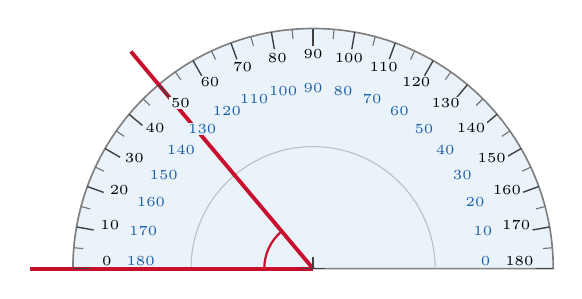
\begin{tikzpicture}
    \def\R{3.05}
    % the plastic
    \fill[protfill] (\R,0) arc[start angle=0, end angle=180, radius=\R] -- cycle;
    \draw[black!50, line width=0.6pt] (\R,0) arc[start angle=0, end angle=180,
      radius=\R] -- cycle;
    \draw[black!25, line width=0.4pt] (1.55,0) arc[start angle=0, end angle=180,
      radius=1.55];
    % the angle: drawn under the numbers, so the numbers stay readable
    \draw[cbred, line width=1.4pt] (0,0) -- (-\R-0.55,0);
    \draw[cbred, line width=1.4pt] (0,0) -- (130:\R+0.55);
    \draw[cbred, line width=0.8pt] (180:0.62) arc[start angle=180, end angle=130,
      radius=0.62];
    % ticks
    \foreach \a in {0,10,...,180} \draw[black!75, line width=0.5pt] (\a:\R) -- (\a:\R-0.22);
    \foreach \a in {5,15,...,175} \draw[black!55, line width=0.4pt] (\a:\R) -- (\a:\R-0.12);
    % outer scale: 0 on the LEFT
    \foreach \a in {0,10,...,180} {
      \pgfmathtruncatemacro{\o}{180-\a}
      \node[font=\tiny, text=black, fill=protfill, inner sep=0.6pt]
        at ($(\a:\R-0.43)+(0,0.1)$) {\o};}
    % inner scale: 0 on the RIGHT
    \foreach \a in {0,10,...,180}
      \node[font=\tiny, text=cbblue, fill=protfill, inner sep=0.6pt]
        at ($(\a:\R-0.86)+(0,0.1)$) {\a};
    % the centre
    \draw[black!75, line width=0.6pt] (-0.15,0) -- (0.15,0) (0,0) -- (0,0.15);
  \end{tikzpicture}
\end{minipage}
\end{minipage}

\vspace{6pt}
\noindent\begin{minipage}{\textwidth}
\noindent\textbf{(d)} How do you know? Finish the sentence. \\[3pt]
\eng{``I count up from the 0 that \ldots''}
\qlines{2}
\end{minipage}

% -- A2 ---------------------------------------------------------------------
% The deck's slide 19 phrases, to match rather than read. The meanings are in
% their own box so no phrase sits beside its answer. Numbers, not letters, for
% the meanings: the phrases already use A, B, C, D and P as points.
\qhead{A2}{The Workbook's words}

\noindent\begin{minipage}{\textwidth}
\noindent Match each question to what it means. Write the \textbf{number} in the box.
(a) is done for you.

\vspace{6pt}
% \vspace{0pt} first in both: a [t] minipage that starts with a box (the
% tcolorbox) takes its baseline from the box's BOTTOM, and the list dropped
% below the whole box.
\noindent\begin{minipage}[t]{0.585\textwidth}\vspace{0pt}\raggedright
  {\renewcommand{\arraystretch}{1.75}%
  \begin{tabular}{@{}l@{\ \ }P{7.1cm}@{\ }l@{}}
    \textbf{(a)} & Draw the line through B perpendicular to AB. & \fbx{4} \\
    \textbf{(b)} & Draw a perpendicular line from C to AB. & \nbox \\
    \textbf{(c)} & Draw a line through P parallel to AB. & \nbox \\
    \textbf{(d)} & Mark the point D. & \nbox \\
    \textbf{(e)} & Measure the length of AD. & \nbox \\
    \textbf{(f)} & How can you check that your answer is correct? & \nbox \\
  \end{tabular}}
\end{minipage}\hfill
\begin{minipage}[t]{0.395\textwidth}\vspace{0pt}
  \begin{tcolorbox}[enhanced, colback=white, colframe=rulegray, boxrule=0.6pt,
                    arc=5pt, left=8pt, right=8pt, top=6pt, bottom=6pt,
                    nobeforeafter]
    \raggedright{\bfseries It means \ldots}
    \begin{enumerate}[label=\textbf{\arabic*}, itemsep=5pt, topsep=4pt]
      \item Use a ruler. Give the length to the nearest mm.
      \item Start at C. Stop on AB. Meet AB at 90\textdegree.
      \item It goes past P. It is always the same distance from AB.
      \item It goes past B, at 90\textdegree\ to AB.
      \item Use a fact, like ``the four angles add up to 360\textdegree''.
      \item Make a small cross. Write D next to it.
    \end{enumerate}
  \end{tcolorbox}
\end{minipage}
\end{minipage}

% -- A3 ---------------------------------------------------------------------
% Parallel and perpendicular with no protractor: count the squares. (a) is
% the deck's "same angle with a line across", as "the same steps". (b) and (c)
% are the slide 19 trap: THROUGH Q (Q is on the line) and FROM C (start at C,
% stop on the line). (e) is the deck's shortest way.
\qhead{A3}{On the grid: parallel and perpendicular}

\noindent\begin{minipage}{\textwidth}
\noindent Use a ruler. Count the squares --- no protractor.

\vspace{6pt}
\noindent\begin{minipage}[t]{0.48\textwidth}\centering
  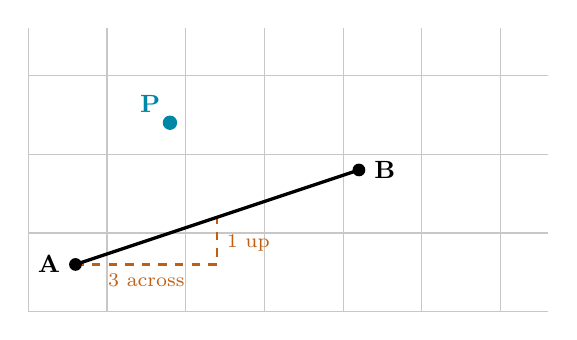
\begin{tikzpicture}[x=0.6cm, y=0.6cm]
    \draw[sq] (0,0) grid (11,6);
    \draw[cborange, line width=0.9pt, dashed] (1,1) -- (4,1) -- (4,2);
    \node[font=\scriptsize, text=cborange, below] at (2.5,1) {3 across};
    \node[font=\scriptsize, text=cborange, right] at (4,1.45) {1 up};
    \draw[line width=1.2pt] (1,1) -- (7,3);
    \fill (1,1) circle (2.3pt); \node[font=\small\bfseries, left=2pt] at (1,1) {A};
    \fill (7,3) circle (2.3pt); \node[font=\small\bfseries, right=2pt] at (7,3) {B};
    \fill[cbteal] (3,4) circle (2.6pt);
    \node[font=\small\bfseries, text=cbteal, above left=0pt] at (3,4) {P};
  \end{tikzpicture}
  \par\vspace{4pt}\raggedright
  \textbf{(a)} Draw the line through \textbf{P} parallel to \textbf{AB}. \\
  {\small AB goes 3 squares across and 1 square up. Your line does the same.}
\end{minipage}\hfill
\begin{minipage}[t]{0.48\textwidth}\centering
  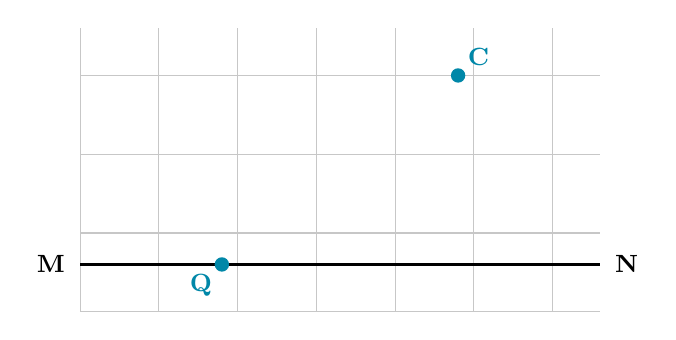
\begin{tikzpicture}[x=0.6cm, y=0.6cm]
    \draw[sq] (0,0) grid (11,6);
    \draw[line width=1.2pt] (0,1) -- (11,1);
    \node[font=\small\bfseries, left=2pt] at (0,1) {M};
    \node[font=\small\bfseries, right=2pt] at (11,1) {N};
    \fill[cbteal] (3,1) circle (2.6pt);
    \node[font=\small\bfseries, text=cbteal, below left=0pt] at (3,1) {Q};
    \fill[cbteal] (8,5) circle (2.6pt);
    \node[font=\small\bfseries, text=cbteal, above right=0pt] at (8,5) {C};
  \end{tikzpicture}
  \par\vspace{4pt}\raggedright
  \textbf{(b)} Draw the line through \textbf{Q} perpendicular to \textbf{MN}. \\
  \textbf{(c)} Draw the perpendicular from \textbf{C} to \textbf{MN}. Mark the point
  \textbf{D} where it meets MN.
\end{minipage}
\end{minipage}

\vspace{8pt}
\noindent\begin{minipage}{\textwidth}
\noindent\textbf{(d)} How many squares long is \textbf{CD}? \ \blank[2.0cm]

\vspace{8pt}
\noindent\textbf{(e)} Mr Bowen walks from C to N. Is that longer or shorter than CD?
Why? \\[3pt] Start: \eng{``CD is the shortest way from C to MN because \ldots''}
\qlines{2}
\end{minipage}

% -- A4 ---------------------------------------------------------------------
% The deck's story (slides 7-8): one nail each, so the frame squashes into a
% rhombus. Four equal sides is not enough; a square needs right angles too.
\qhead{A4}{A square needs right angles}

\noindent\begin{minipage}{\textwidth}
\noindent Mr Bowen makes a square frame from four sticks. Each stick is 40 cm long.
He puts \textbf{one} nail in each corner. Then he pushes it.

\vspace{6pt}
\noindent\begin{minipage}[c]{0.47\textwidth}\centering
  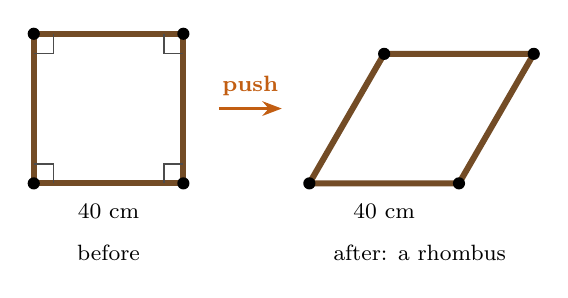
\begin{tikzpicture}[line width=2.2pt, brown!60!black]
    \draw (0,0) rectangle (1.9,1.9);
    \foreach \p in {(0,0),(1.9,0),(1.9,1.9),(0,1.9)} \fill[black] \p circle (2.2pt);
    \draw[black!70, line width=0.6pt] (0.25,0) -- (0.25,0.25) -- (0,0.25);
    \draw[black!70, line width=0.6pt] (1.65,0) -- (1.65,0.25) -- (1.9,0.25);
    \draw[black!70, line width=0.6pt] (1.65,1.9) -- (1.65,1.65) -- (1.9,1.65);
    \draw[black!70, line width=0.6pt] (0.25,1.9) -- (0.25,1.65) -- (0,1.65);
    \node[black, font=\footnotesize, below=3pt] at (0.95,0) {40 cm};
    \node[black, font=\footnotesize, below=18pt] at (0.95,0) {before};
    \draw[cborange, line width=1.1pt, -{Stealth[length=7pt]}] (2.35,0.95) -- (3.15,0.95);
    \node[cborange, font=\footnotesize\bfseries, above] at (2.75,0.95) {push};
    \begin{scope}[xshift=3.5cm]
      \draw (0,0) -- (1.9,0) -- (2.85,1.645) -- (0.95,1.645) -- cycle;
      \foreach \p in {(0,0),(1.9,0),(2.85,1.645),(0.95,1.645)}
        \fill[black] \p circle (2.2pt);
      \node[black, font=\footnotesize, below=3pt] at (0.95,0) {40 cm};
      \node[black, font=\footnotesize, below=18pt] at (1.4,0) {after: a rhombus};
    \end{scope}
  \end{tikzpicture}
\end{minipage}\hfill
\begin{minipage}[c]{0.50\textwidth}
  \noindent\textbf{(a)} Tick (\checkmark) each box that is true.

  \vspace{4pt}
  {\renewcommand{\arraystretch}{1.5}%
  \noindent\begin{tabular}{|l|C{2.25cm}|C{2.25cm}|}
    \hline
    \textbf{Shape} & \textbf{4 equal sides} & \textbf{4 right angles} \\ \hline
    square \tall & & \\ \hline
    rhombus \tall & & \\ \hline
    rectangle \tall & & \\ \hline
  \end{tabular}}
\end{minipage}

\vspace{10pt}
\noindent\textbf{(b)} Mr Bowen says: \emph{``My frame still has four sides of 40 cm. So it
is still a square.''} Is he right? Answer in a full sentence. \\[3pt]
Start: \eng{``No, because a square also needs \ldots''}
\qlines{2}
\end{minipage}

% -- A5 ---------------------------------------------------------------------
% The deck's check (slide 18) and its exit question: add the four measured
% angles; 360 is accurate. Then the table (slide 22) with new numbers and an
% angle that is not 90: the outside is 250, so the inside is 110, and the
% check closes it.
\qhead{A5}{Does it add up to 360\textdegree?}

\noindent\begin{minipage}{\textwidth}
\noindent\textbf{(a)} Mr Bowen draws four quadrilaterals. He measures the four angles of each one.
Add them up. Is the drawing \textbf{accurate}? Row 1 is done for you.

\vspace{4pt}
{\renewcommand{\arraystretch}{1.4}%
\noindent\begin{tabularx}{\textwidth}{|C{1.6cm}|C{4.2cm}|L|C{2.4cm}|}
  \hline
  \textbf{Drawing} & \textbf{The four angles} & \textbf{Add them up} &
    \textbf{Accurate?} \\ \hline
  1 \tall & $85\dg,\ 95\dg,\ 100\dg,\ 80\dg$ &
    \leavevmode{\color{cbteal}$85 + 95 + 100 + 80 = 360\dg$} & {\color{cbteal}yes} \\ \hline
  2 \tall & $70\dg,\ 120\dg,\ 110\dg,\ 50\dg$ & & yes \sep no \\ \hline
  3 \tall & $64\dg,\ 116\dg,\ 64\dg,\ 116\dg$ & & yes \sep no \\ \hline
  4 \tall & $90\dg,\ 90\dg,\ 90\dg,\ 100\dg$ & & yes \sep no \\ \hline
\end{tabularx}}
\end{minipage}

\vspace{10pt}
\noindent\begin{minipage}{\textwidth}
\noindent\begin{minipage}[c]{0.40\textwidth}\centering
  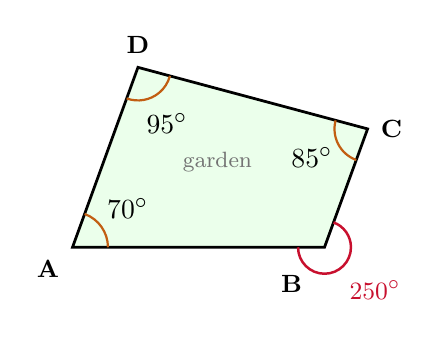
\begin{tikzpicture}[line width=1pt, scale=0.8]
    \coordinate (A) at (0,0); \coordinate (B) at (4,0);
    \coordinate (C) at (4.684,1.879); \coordinate (D) at (1.039,2.856);
    \fill[green!8] (A) -- (B) -- (C) -- (D) -- cycle;
    \draw (A) -- (B) -- (C) -- (D) -- cycle;
    \pic[ang, "$70\dg$", angle radius=0.45cm, angle eccentricity=1.9] {angle = B--A--D};
    \pic[ang, "$85\dg$", angle eccentricity=1.9] {angle = D--C--B};
    \pic[ang, "$95\dg$", angle eccentricity=1.9] {angle = A--D--C};
    \draw[cbred, line width=0.9pt] ($(B)+(180:0.42)$) arc[start angle=180,
      end angle=430, radius=0.42];
    \node[font=\small, text=cbred] at ($(B)+(320:1.05)$) {$250\dg$};
    % B's letter sits outside the red arc, below left
    \node[font=\small\bfseries] at ($(B)+(228:0.78)$) {B};
    \foreach \p/\l/\pos in {A/A/below left, C/C/right, D/D/above}
      \node[font=\small\bfseries, \pos=1pt] at (\p) {\l};
    \node[font=\footnotesize, text=black!55] at (2.3,1.35) {garden};
  \end{tikzpicture}
\end{minipage}\hfill
\begin{minipage}[c]{0.57\textwidth}\raggedright
  \textbf{(b)} This is Mr Bowen's garden. He measures the angle at \textbf{B} and reads
  \textbf{250\textdegree}.

  \vspace{6pt}
  \textbf{(i)} Did he measure the inside or the outside? \ \blank[2.4cm]

  \vspace{8pt}
  \textbf{(ii)} What is the angle \textbf{inside} the garden at B?
  \par\vspace{6pt}\textbf{Calculation:} \blank[3.4cm] \ \textbf{Answer:} \blank[1.6cm]
\end{minipage}

\vspace{8pt}
\noindent\textbf{(iii)} Check: do the four angles inside the garden add up to
360\textdegree? Write the calculation.
\par\vspace{8pt}\noindent\hspace*{1.6em}\blank[11cm]
\end{minipage}

% ===========================================================================
% SECTION B -- REVIEW OF 5.1 AND 5.2
% ===========================================================================
\hwsection{Section B \textperiodcentered\ Review of 5.1 and 5.2 --- Calculate, Do Not
Measure}

% -- B1 ---------------------------------------------------------------------
% Four facts: round a point, vertically opposite, corresponding (F), alternate
% (Z, and obtuse this time). The straight line and the quadrilateral were cut
% to reach eight pages; A5 already does 360 in a quadrilateral. All six
% reasons stay in the box, so the last one cannot be found by elimination.
\qhead{B1}{Find the angle. Give a reason.}

\begin{wordhelp}[The reasons --- copy the one you need after \textbf{because}]
  \renewcommand{\arraystretch}{1.2}%
  \begin{tabularx}{\linewidth}{@{}p{8.4cm}L@{}}
    \textbf{line:} angles on a straight line add up to 180\textdegree &
    \textbf{X:} vertically opposite angles are equal \\
    \textbf{point:} angles around a point add up to 360\textdegree &
    \textbf{F:} corresponding angles are equal \\
    \textbf{shape:} angles in a quadrilateral add up to 360\textdegree &
    \textbf{Z:} alternate angles are equal \\
  \end{tabularx}
\end{wordhelp}

\noindent\begin{minipage}{\textwidth}
\noindent Arrows ($>$) on two lines mean they are \textbf{parallel}. Calculate each
letter. Then give a reason.

\vspace{6pt}
\noindent
\begin{minipage}[b]{0.235\textwidth}\centering
  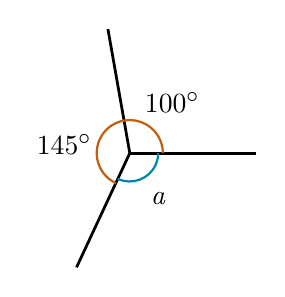
\begin{tikzpicture}[line width=1pt]
    \coordinate (O) at (0,0); \coordinate (R) at (0:1.6);
    \coordinate (P) at (100:1.6); \coordinate (Q) at (245:1.6);
    \draw (O) -- (R); \draw (O) -- (P); \draw (O) -- (Q);
    \pic[ang, "$100\dg$", angle eccentricity=2.0] {angle = R--O--P};
    \pic[ang, "$145\dg$", angle eccentricity=2.0] {angle = P--O--Q};
    \pic[let, "$a$", angle eccentricity=1.9] {angle = Q--O--R};
  \end{tikzpicture}\par\vspace{2pt}\textbf{(a)}
\end{minipage}\hfill
\begin{minipage}[b]{0.235\textwidth}\centering
  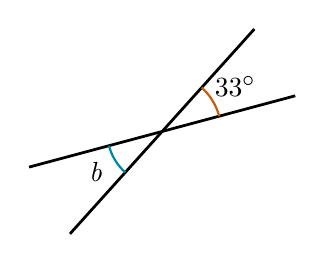
\begin{tikzpicture}[line width=1pt]
    \coordinate (O) at (0,0);
    \coordinate (A1) at (15:1.75); \coordinate (A2) at (195:1.75);
    \coordinate (B1) at (48:1.75); \coordinate (B2) at (228:1.75);
    \draw (A2) -- (A1); \draw (B2) -- (B1);
    \pic[ang, "$33\dg$", angle radius=0.75cm, angle eccentricity=1.45] {angle = A1--O--B1};
    \pic[let, "$b$", angle radius=0.7cm, angle eccentricity=1.4] {angle = A2--O--B2};
  \end{tikzpicture}\par\vspace{2pt}\textbf{(b)}
\end{minipage}\hfill
\begin{minipage}[b]{0.235\textwidth}\centering
  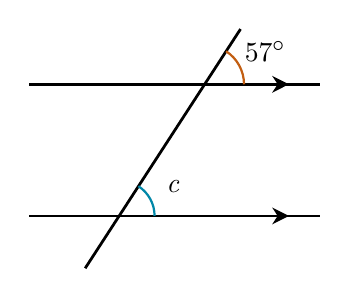
\begin{tikzpicture}[line width=1pt, scale=0.88]
    \draw (0,0) -- (4.2,0); \draw (0,1.9) -- (4.2,1.9);
    \draw[par] (3.5,0) -- (3.75,0); \draw[par] (3.5,1.9) -- (3.75,1.9);
    \coordinate (B) at (1.3,0); \coordinate (T) at (2.534,1.9);
    \coordinate (TR) at (4.2,1.9); \coordinate (TU) at (3.052,2.697);
    \coordinate (BR) at (4.2,0);
    \draw (0.81,-0.755) -- (TU);
    \pic[ang, "$57\dg$", angle radius=0.5cm, angle eccentricity=1.75] {angle = TR--T--TU};
    \pic[let, "$c$", angle radius=0.45cm, angle eccentricity=1.75] {angle = BR--B--T};
  \end{tikzpicture}\par\vspace{2pt}\textbf{(c)}
\end{minipage}\hfill
\begin{minipage}[b]{0.235\textwidth}\centering
  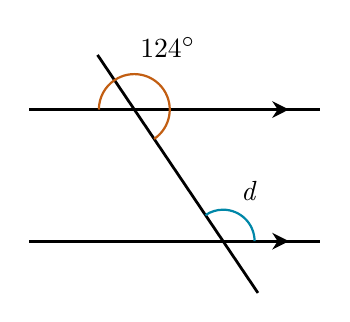
\begin{tikzpicture}[line width=1pt, scale=0.88]
    \draw (0,0) -- (4.2,0); \draw (0,1.9) -- (4.2,1.9);
    \draw[par] (3.5,0) -- (3.75,0); \draw[par] (3.5,1.9) -- (3.75,1.9);
    \coordinate (B) at (2.8,0); \coordinate (T) at (1.519,1.9);
    \coordinate (TL) at (0,1.9); \coordinate (BR) at (4.2,0);
    \draw (3.303,-0.746) -- (0.988,2.688);
    \pic[ang, "$124\dg$", angle radius=0.45cm, angle eccentricity=2.0] {angle = B--T--TL};
    \pic[let, "$d$", angle radius=0.4cm, angle eccentricity=1.8] {angle = BR--B--T};
  \end{tikzpicture}\par\vspace{2pt}\textbf{(d)}
\end{minipage}
\end{minipage}

% The answer table is its own block, so the diagrams can end one page and the
% table start the next. A tabular never splits by itself.
\vspace{8pt}
\noindent\begin{minipage}{\textwidth}
{\renewcommand{\arraystretch}{1.6}%
\noindent\begin{tabular}{@{}l@{\ }l@{\ \ }l@{}}
  $a =$ & \blank[1.5cm] & because \blank[10.6cm] \\
  $b =$ & \blank[1.5cm] & because \blank[10.6cm] \\
  $c =$ & \blank[1.5cm] & because \blank[10.6cm] \\
  $d =$ & \blank[1.5cm] & because \blank[10.6cm] \\
\end{tabular}}
\end{minipage}

% ===========================================================================
% SECTION C -- SCIENCE 4.1: CHARACTERISTICS OF LIVING ORGANISMS
% ===========================================================================
\hwsection[cbgreen]{Section C \textperiodcentered\ Science 4.1 --- Characteristics of
Living Organisms}

% -- C1 ---------------------------------------------------------------------
% The four write panels, word for word. Meanings in their own box, so no word
% sits next to its letter (the HW 10 lesson).
\qhead[cbgreen]{C1}{The seven, and one more}

\noindent\begin{minipage}{\textwidth}
\noindent Match each word to its meaning. Write the \textbf{letter} in the box. The
first one is done for you.

\vspace{6pt}
\begin{tcolorbox}[enhanced, colback=white, colframe=rulegray, boxrule=0.6pt, arc=5pt,
                  left=8pt, right=8pt, top=4pt, bottom=4pt]
  \renewcommand{\arraystretch}{1.12}%
  \begin{tabularx}{\linewidth}{@{}p{0.45cm}L p{0.45cm}L@{}}
    \textbf{A} & a living thing &
    \textbf{E} & changing position or shape \\
    \textbf{B} & getting bigger &
    \textbf{F} & taking in or making food \\
    \textbf{C} & noticing changes around it &
    \textbf{G} & making more organisms of the same kind \\
    \textbf{D} & getting rid of waste, such as carbon dioxide &
    \textbf{H} & breaking down food inside cells to get energy \\
  \end{tabularx}
\end{tcolorbox}

\vspace{4pt}
{\renewcommand{\arraystretch}{1.6}%
\noindent\begin{tabularx}{\textwidth}{@{}L L L L@{}}
  organism \fbx{A} & movement \nbox & respiration \nbox & sensitivity \nbox \\
  growth \nbox & reproduction \nbox & excretion \nbox & nutrition \nbox \\
\end{tabularx}}
\end{minipage}

% -- C2 ---------------------------------------------------------------------
% A new animal for the polar bear's seven labels: a gecko on the classroom
% wall. Row 8 is deadpan, and has two answers.
\qhead[cbgreen]{C2}{The gecko on the wall}

\noindent\begin{minipage}{\textwidth}
\noindent A gecko lives on the wall of Mr Bowen's classroom. Which of the seven is each
clue? Row 1 is done for you.

\vspace{4pt}
\noindent\begin{tabularx}{\textwidth}{|L|P{4.5cm}|}
  \hline
  \textbf{Clue} & \textbf{Which of the seven?} \\ \hline
  1. The gecko runs up the wall. \tall & {\color{cbteal}movement} \\ \hline
  2. It sees a fly and turns its head. \tall & \\ \hline
  3. It eats the fly. \tall & \\ \hline
  4. Inside its cells, the fly is broken down to give energy. \tall & \\ \hline
  5. It breathes out carbon dioxide. \tall & \\ \hline
  6. It lays two eggs. \tall & \\ \hline
  7. A baby gecko is 3 cm long. A month later, it is 5 cm long. \tall & \\ \hline
  8. The gecko falls onto Mr Bowen's desk. Mr Bowen sees it and jumps. \textbf{Name
     two} of the seven that Mr Bowen does. \tall & \\ \hline
\end{tabularx}
\end{minipage}

% -- C3 ---------------------------------------------------------------------
% The respiration vote (breathing is not respiration), the tree that does not
% breathe, the jog, and the two meanings of "sensitive".
\qhead[cbgreen]{C3}{Breathing or respiration?}

\noindent\begin{minipage}{\textwidth}
\noindent Tick (\checkmark) \textbf{true} or \textbf{false}.

\vspace{4pt}
{\renewcommand{\arraystretch}{1.3}%
\noindent\begin{tabularx}{\textwidth}{|L|C{1.6cm}|C{1.6cm}|}
  \hline
  & \textbf{True} & \textbf{False} \\ \hline
  1. Respiration is the same as breathing. \tall & & \\ \hline
  2. Respiration happens inside cells. \tall & & \\ \hline
  3. Breathing brings in the oxygen that respiration uses. \tall & & \\ \hline
  4. A tree does not breathe in and out like us, so it does not do respiration.
     \tall & & \\ \hline
  5. When you run, your cells do more respiration. \tall & & \\ \hline
  6. In science, \textbf{sensitive} means ``gets upset easily''. \tall & & \\ \hline
\end{tabularx}}

\vspace{8pt}
\noindent Choose \textbf{one} false sentence. Write it again so that it is true.
\qlines{1}
\end{minipage}

% -- C4 ---------------------------------------------------------------------
% The game's traps with new things: a seed (alive, resting), wood and cotton
% and paper (alive once), a river (moves and grows), a candle flame (fire),
% mould (alive).
\qhead[cbgreen]{C4}{Alive, alive once, or never alive?}

\noindent\begin{minipage}{\textwidth}
\begin{wordhelp}
  \textbf{Alive:} it is a living organism now. \quad \textbf{Alive once:} it came from
  a living thing, but it is not alive now (a wooden desk was a tree). \quad
  \textbf{Never alive:} it was never a living thing.
\end{wordhelp}

\noindent Write \textbf{A} (alive), \textbf{O} (alive once) or \textbf{N} (never alive)
in each box.

\vspace{4pt}
{\renewcommand{\arraystretch}{1.85}%
\noindent\begin{tabularx}{\textwidth}{@{}L L L@{}}
  a mango tree \nbox & a wooden pencil \nbox & a river \nbox \\
  a mango seed \nbox & a candle flame \nbox & a cotton T-shirt \nbox \\
  mould on old bread \nbox & a glass bottle \nbox & a sheet of paper \nbox \\
\end{tabularx}}
\end{minipage}

\vspace{8pt}
\noindent\begin{minipage}{\textwidth}
\noindent Mr Bowen says: \emph{``The river is alive. It moves, and it gets bigger in the
rainy season.''} Is he right? Answer in full sentences. \\[3pt]
Start: \eng{``No. A river moves and gets bigger, but it does not \ldots''}
\qlines{2}
\end{minipage}

% -- C5 ---------------------------------------------------------------------
% The car and the robot vacuum again, as a robot dog: some of the seven, sort
% of, but not all. Then the other way round: a cactus does not seem to do
% much, and it does all seven. The write panel is the tool for both.
\qhead[cbgreen]{C5}{The robot dog and the cactus}

\begin{remember}[Remember from the lesson]
  A living organism does \key{all seven}. A non-living thing may do some, but
  \key{not all}.
\end{remember}

\noindent\begin{minipage}{\textwidth}
\noindent Mr Bowen buys a robot dog. It walks around the room. It barks when someone
comes in. When its battery is low, it goes to its charger. It never gets bigger. Mr
Bowen says it loves him.

\vspace{6pt}
\noindent\textbf{(a)} Is the robot dog alive? Answer in full sentences. Name \textbf{two}
of the seven it seems to do, and \textbf{two} it \textbf{cannot} do. \\[3pt]
Start: \eng{``The robot dog seems to do \ldots\ But it is not alive because it cannot
\ldots''}
\qlines{3}
\end{minipage}

\vspace{8pt}
\noindent\begin{minipage}{\textwidth}
\noindent\textbf{(b)} A cactus does not walk, and it does not eat. But it \textbf{is}
alive. Explain, in full sentences. Name \textbf{three} of the seven that a cactus does.
\\[3pt]
Start: \eng{``A cactus makes its own food using light, so \ldots''}
\qlines{3}
\end{minipage}

% ===========================================================================
% SECTION D -- SCIENCE 4.2: VIRUSES
% ===========================================================================
\hwsection[cbgreen]{Section D \textperiodcentered\ Science 4.2 --- Viruses}

% -- D1 ---------------------------------------------------------------------
% The deck's drawing (slide 8), to label instead of copy. The peg and the coat
% are next to each other on a virus, so their leaders leave on opposite
% sides: the peg leader is horizontal to a peg's head on the left, the coat
% leader goes out between two pegs on the lower right.
\qhead[cbgreen]{D1}{Label the virus}

\noindent\begin{minipage}{\textwidth}
\noindent Label each part: \textbf{pegs} \sep\ \textbf{protein coat} \sep\
\textbf{RNA}. The grey words say what it does.

\vspace{6pt}
{\centering
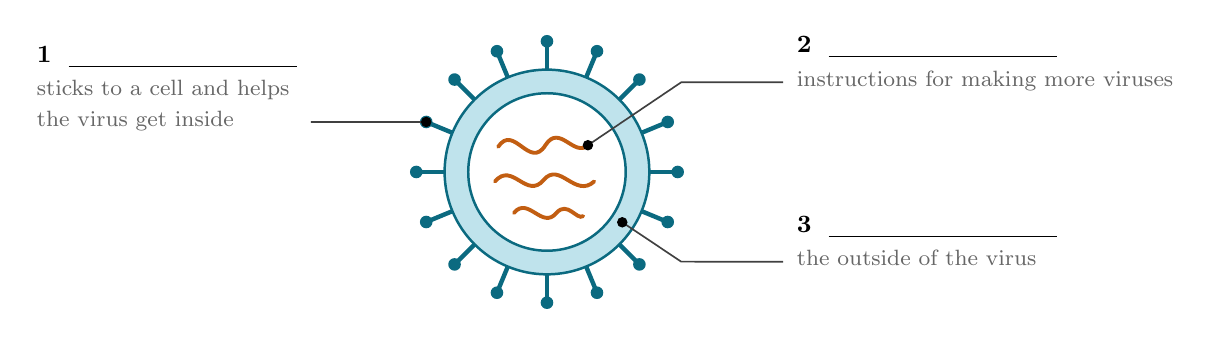
\begin{tikzpicture}
  % pegs
  \foreach \a in {0,22.5,...,337.5} {
    \draw[coatline, line width=1.6pt] (\a:1.28) -- (\a:1.6);
    \fill[coatline] (\a:1.66) circle (0.08);}
  % the coat
  \fill[coatfill] (0,0) circle (1.3);
  \fill[white] (0,0) circle (1.0);
  \draw[coatline, line width=0.9pt] (0,0) circle (1.3);
  \draw[coatline, line width=0.9pt] (0,0) circle (1.0);
  % RNA
  \draw[cborange, line width=1.4pt, line cap=round]
    (-0.62,0.32) .. controls (-0.42,0.62) and (-0.22,0.02) .. (-0.02,0.34)
    .. controls (0.16,0.62) and (0.34,0.18) .. (0.52,0.34);
  \draw[cborange, line width=1.4pt, line cap=round]
    (-0.66,-0.12) .. controls (-0.44,0.14) and (-0.26,-0.36) .. (-0.04,-0.1)
    .. controls (0.16,0.14) and (0.36,-0.34) .. (0.6,-0.12);
  \draw[cborange, line width=1.4pt, line cap=round]
    (-0.42,-0.52) .. controls (-0.24,-0.3) and (-0.06,-0.74) .. (0.12,-0.52)
    .. controls (0.26,-0.36) and (0.38,-0.62) .. (0.46,-0.56);
  % leader 1: a peg (horizontal, to the head of the peg at 157.5 degrees)
  \draw[lead] (-3.0,0.635) -- (157.5:1.66);
  \fill[black] (157.5:1.66) circle (1.9pt);
  \node[anchor=base east, font=\small, align=left] at (-3.05,0.58)
    {\textbf{1} \ \blank[2.9cm]\\[1pt]{\footnotesize\color{black!60}sticks to a cell and
    helps}\\{\footnotesize\color{black!60}the virus get inside}};
  % leader 2: the RNA (out between the pegs at 22.5 and 45 degrees)
  \draw[lead] (0.52,0.34) -- (33.75:2.05) -- (3.0,1.14);
  \fill[black] (0.52,0.34) circle (1.9pt);
  \node[anchor=base west, font=\small, align=left] at (3.05,1.09)
    {\textbf{2} \ \blank[2.9cm]\\[1pt]{\footnotesize\color{black!60}instructions for making
    more viruses}};
  % leader 3: the coat (out between the pegs at -22.5 and -45 degrees)
  \draw[lead] (-33.75:1.15) -- (-33.75:2.05) -- (3.0,-1.14);
  \fill[black] (-33.75:1.15) circle (1.9pt);
  \node[anchor=base west, font=\small, align=left] at (3.05,-1.19)
    {\textbf{3} \ \blank[2.9cm]\\[1pt]{\footnotesize\color{black!60}the outside of the
    virus}};
\end{tikzpicture}\par}
\end{minipage}

% -- D2 ---------------------------------------------------------------------
% Slides 4-7: the cell's three parts that a virus does not have, the two
% microscopes, respiration (4.1 again). Row 6 is the only "both".
\qhead[cbgreen]{D2}{A cell or a virus?}

\noindent\begin{minipage}{\textwidth}
\noindent Tick (\checkmark) the \textbf{cell}, the \textbf{virus}, or \textbf{both}.

\vspace{4pt}
{\renewcommand{\arraystretch}{1.3}%
\noindent\begin{tabularx}{\textwidth}{|L|C{2.9cm}|C{2.4cm}|}
  \hline
  & \textbf{A cell in Mr Bowen's nose} & \textbf{A flu virus} \\ \hline
  1. It has a cell membrane, cytoplasm and a nucleus. \tall & & \\ \hline
  2. It has a protein coat with pegs. \tall & & \\ \hline
  3. You can see it with a school microscope. \tall & & \\ \hline
  4. You can only see it with an electron microscope. \tall & & \\ \hline
  5. It does respiration. \tall & & \\ \hline
  6. You cannot see it with your eyes alone. \tall & & \\ \hline
\end{tabularx}}
\end{minipage}

% -- D3 ---------------------------------------------------------------------
% The flu model's five verbs (slide 11) as five sentences, shuffled. (b) is
% the copying vote (slide 9) and Be the Cell: the CELL makes the copies.
% (c) is the book's "this makes the animal ... feel ill".
\qhead[cbgreen]{D3}{Follow the flu virus}

\begin{wordhelp}
  \eng{replicate}: make copies \quad\sep\quad \eng{burst}: break open suddenly
  \quad\sep\quad \eng{flu}: short for \textbf{influenza}
\end{wordhelp}

\noindent\begin{minipage}{\textwidth}
\noindent\textbf{(a)} A flu virus replicates. Put the steps in order: write
\textbf{1} to \textbf{5}. Step 1 is done for you.

\vspace{4pt}
{\renewcommand{\arraystretch}{1.5}%
\noindent\begin{tabular}{@{}l l@{}}
  \nbox & The cell copies the RNA. It builds many new viruses. \\
  \fbx{1} & The pegs stick to a cell in the nose. \\
  \nbox & The cell bursts and dies. The new viruses float away. \\
  \nbox & The virus gets inside the cell. \\
  \nbox & The virus bursts open. Its RNA comes out. \\
\end{tabular}}
\end{minipage}

\vspace{8pt}
\noindent\begin{minipage}{\textwidth}
\noindent\textbf{(b)} Mr Bowen says: \emph{``A virus makes copies of itself, like a
photocopier.''} What is wrong with this? \\[3pt]
Start: \eng{``The virus does not make the copies. The \ldots''}
\qlines{3}
\end{minipage}

\vspace{6pt}
\noindent\begin{minipage}{\textwidth}
\noindent\textbf{(c)} Why do you feel ill when you have flu? \\[3pt]
Start: \eng{``When the new viruses burst out, the cells \ldots''}
\qlines{3}
\end{minipage}

% -- D4 ---------------------------------------------------------------------
% The book's Think like a scientist (page 132), as a question: clay, pins,
% threads. (b) is what a model gets wrong: size (0.0001 mm), colour (added in
% the photos), material.
\qhead[cbgreen]{D4}{Mr Bowen's model virus}

\noindent\begin{minipage}{\textwidth}
\noindent Mr Bowen makes a model of a flu virus. He uses a ball of green modelling clay,
20 push pins, and short pieces of red wool, pushed inside the clay.

\vspace{4pt}
\noindent\begin{minipage}[t]{0.47\textwidth}
\noindent\textbf{(a)} What is each part of the model?

\vspace{4pt}
{\renewcommand{\arraystretch}{1.3}%
\noindent\begin{tabular}{|P{2.9cm}|P{3.5cm}|}
  \hline
  \textbf{In the model} & \textbf{In a real virus} \\ \hline
  the green clay ball \tall & \\ \hline
  the push pins \tall & \\ \hline
  the red wool \tall & \\ \hline
\end{tabular}}
\end{minipage}\hfill
\begin{minipage}[t]{0.49\textwidth}
\noindent\textbf{(b)} Give \textbf{one} way the model is \textbf{not} like a real
virus. \\[3pt]
Start: \eng{``A real virus is \ldots''}
\qlines{3}
\end{minipage}
\end{minipage}

% -- D5 ---------------------------------------------------------------------
% The deck's slides 15-17: the virus against the seven (six no, one sort of),
% then the writing, from the book's Activity 4.2.1 sentence frame. Last, and
% atomic: it is the full-page-ish block that strands space if it sits mid-way.
\qhead[cbgreen]{D5}{Is a virus alive?}

\noindent\begin{minipage}{\textwidth}
\noindent\textbf{(a)} On its own, outside a cell, does a virus do each of the seven? Write
\textbf{Y} (yes), \textbf{N} (no) or \textbf{S} (sort of).

\vspace{6pt}
{\renewcommand{\arraystretch}{1.4}%
\noindent\begin{tabularx}{\textwidth}{@{}L L L L@{}}
  movement \nbox & respiration \nbox & sensitivity \nbox & growth \nbox \\
  reproduction \nbox & excretion \nbox & nutrition \nbox & \\
\end{tabularx}}
\end{minipage}

\vspace{8pt}
\noindent\begin{minipage}{\textwidth}
\noindent\textbf{(b)} Some scientists say a virus is alive. Others say it is not. What do
\textbf{you} think? Write 5 sentences. \\[3pt]
Start: \eng{``I think a virus is / is not alive because \ldots''}

\begin{yourturn}[Your answer must have: tick each one]
  \renewcommand{\arraystretch}{1.35}%
  \begin{tabularx}{\linewidth}{@{}p{0.75cm}L p{0.75cm}L p{0.75cm}L@{}}
    \tickbox & what \textbf{you} think, and \textbf{because} & \tickbox & a reason for
      the \textbf{other} side & \tickbox & the word \textbf{cells} \\
    \tickbox & the word \textbf{replicate} & \tickbox & one of the \textbf{seven}, by
      name & \tickbox & full sentences \\
  \end{tabularx}
\end{yourturn}
\wlines{7}
\end{minipage}

% ===========================================================================
% ANSWER KEY -- TEACHER COPY ONLY
% ===========================================================================
\ifkey
\clearpage

\hwsection[cbred]{Answer Key --- Teacher Copy}

\linespread{1.0}\selectfont
\setlist[enumerate]{itemsep=2pt, topsep=3pt, leftmargin=*}
\setlist[itemize]{itemsep=2pt, topsep=3pt, leftmargin=*}

\qhead[cbred]{A1}{Read the protractor}
\noindent (a) acute \quad (b) 50 and 130 \quad (c) $\mathbf{50\dg}$ \\
(d) \emph{I count up from the 0 that sits on the line (the outside scale). The angle is
acute, so it is less than 90\textdegree.}

\smallskip
\noindent{\small 130\textdegree\ is the deck's vote and the commonest error: the
student read the scale whose 0 is on the \emph{other} side. The estimate in (a) is
there to catch it --- an acute angle cannot be 130\textdegree. A student who writes
``acute'' and then 130 has not connected the two: point at their own answer to (a).}

\qhead[cbred]{A2}{The Workbook's words}
\noindent (a) 4 \quad (b) 2 \quad (c) 3 \quad (d) 6 \quad (e) 1 \quad (f) 5

\smallskip
\noindent{\small (a) and (b) are the pair that matters: \emph{through} B means the line
passes B; \emph{from} C \emph{to} AB means start at C and stop on AB. A student who
swaps 2 and 4 will draw A3(b) and A3(c) the wrong way round too.}

\qhead[cbred]{A3}{On the grid}
\noindent (a) Any line through P that goes 3 across and 1 up, e.g.\ through (0,\,3),
P (3,\,4), (6,\,5) and (9,\,6), counting squares from the bottom left. \\
(b) The vertical line through Q. \quad (c) The vertical line from C down to MN; D is
4 squares below C. \quad (d) \textbf{4} squares. \\
(e) \emph{CN is longer. CD is the shortest way from C to MN because it meets MN at
90\textdegree.}

\smallskip
\noindent{\small (a) Check the gap: the two lines are the same number of squares apart
at both ends. Expect a line that goes 1 across and 3 up (the steps swapped) --- it
crosses AB, so it cannot be parallel; and a flat line through P, which ``looks
parallel'' only because AB is not steep. \\
(b) and (c) are the same drawing move and different English. A student whose line
for (b) runs from Q up to C has read \emph{through Q} as \emph{from Q to C}. A line for
(c) that ends at Q (not straight down) has the perpendicular wrong: ask what angle
it makes with MN. \\
(e) CN is 5 squares (3 across, 4 down); nobody needs the number. The reason is the write panel:
90\textdegree\ and shortest.}

\qhead[cbred]{A4}{A square needs right angles}
\noindent (a) square: \checkmark\ \checkmark \quad rhombus: \checkmark\ (sides only)
\quad rectangle: \checkmark\ (right angles only) \\
(b) \emph{No, because a square also needs four right angles. The corners turned, so
the frame is now a rhombus.}

\smallskip
\noindent{\small The rectangle's ``4 equal sides'' box: accept it left blank. A student
who ticks it is thinking of a square, which is a special rectangle; that is fine to
discuss, not to mark wrong. \\
(b) A student who agrees with Mr Bowen has kept only half the definition. The deck's
fix is the rulers: four equal sides, pushed, still four equal sides.}

\qhead[cbred]{A5}{Does it add up to 360\textdegree?}
\noindent 2: $70 + 120 + 110 + 50 = 350\dg$, \textbf{no} \quad 3: $64 + 116 + 64 + 116 =
360\dg$, \textbf{yes} \quad 4: $90 + 90 + 90 + 100 = 370\dg$, \textbf{no} \\
(b)(i) the outside \quad (ii) $360 - 250 = \mathbf{110\dg}$ \quad (iii) $110 + 70 + 85 +
95 = 360\dg$: yes.

\smallskip
\noindent{\small Drawing 4 is three right angles and one that is not: a student who says
``yes'' saw a rectangle and did not add. \\
(b) is the deck's table (270\textdegree) with an angle that is not a right angle.
Expect $250 - 180 = 70$ from a student who reaches for 180: the red arc goes all the
way round the outside, so it is 360. (iii) is the payoff: the 110 they found makes the
four add up, which is how they know (ii) is right.}

\qhead[cbred]{B1}{Find the angle. Give a reason.}
\noindent $a = 115\dg$ because angles around a point add up to $360\dg$ ($360 - 100 - 145$). \\
$b = 33\dg$ because vertically opposite angles are equal. \\
$c = 57\dg$ because corresponding angles are equal. \\
$d = 124\dg$ because alternate angles are equal.

\smallskip
\noindent{\small Accept the reason in the student's own words if the fact is right
(``they make a Z'' is fine for $d$). A number with no reason is half done. \\
(a) Expect $180 - 245$, which cannot be done, from anyone who uses 180 for everything:
ask ``180 or 360?'' \\
(b) Expect $147\dg$ from a student who took the angle \emph{next to} $33\dg$. \\
(d) is obtuse on purpose. Expect $56\dg$ ($180 - 124$) from a student who believes
alternate angles are always the small ones. \\
The straight line and the quadrilateral are not repeated here: A5 already uses
360\textdegree\ in a quadrilateral twice.}

\qhead[cbred]{C1}{The seven, and one more}
\noindent movement \textbf{E} \quad respiration \textbf{H} \quad sensitivity \textbf{C}
\quad growth \textbf{B} \quad reproduction \textbf{G} \quad excretion \textbf{D} \quad
\mbox{nutrition \textbf{F}}

\smallskip
\noindent{\small These are the four write panels word for word, so a student with a
complete notebook can check every one. Respiration and excretion are the pair most
often swapped (both involve gases).}

\qhead[cbred]{C2}{The gecko on the wall}
\noindent 2 sensitivity \quad 3 nutrition \quad 4 respiration \quad 5 excretion \quad 6
reproduction \quad 7 growth \quad 8 sensitivity and movement

\smallskip
\noindent{\small 4 is the one to watch: ``breathing'' is not one of the seven, and the
clue says \emph{inside its cells}. 5 is excretion, not respiration --- the waste
leaving. 8 is deadpan; Mr Bowen noticed a change (sensitivity) and jumped (movement).
Accept respiration as a third.}

\qhead[cbred]{C3}{Breathing or respiration?}
\noindent 1 false \quad 2 true \quad 3 true \quad 4 false \quad 5 true \quad 6 false \\
Corrected, any one: \emph{Respiration is not the same as breathing.} / \emph{A tree does
respiration in its cells, even though it does not breathe like us.} / \emph{In science,
sensitive means noticing changes around it.}

\smallskip
\noindent{\small Expect most of the class to get 1 wrong: it is the deck's vote
(slide 7), and French has the same trap. 4 is the book's own sentence turned round:
``Plants don't breathe or have hearts, yet they are alive.'' A correction that just
adds ``not'' is fine if the sentence is now true.}

\qhead[cbred]{C4}{Alive, alive once, or never alive?}
\noindent \textbf{A:} mango tree, mango seed, mould \quad \textbf{O:} wooden pencil,
cotton T-shirt, sheet of paper \quad \textbf{N:} river, candle flame, glass bottle \\
\emph{No. A river moves and gets bigger, but it does not eat, respire or reproduce. A
living organism does all seven, so a river is not alive.}

\smallskip
\noindent{\small The traps, in the order the game taught them: the seed is alive (it is
resting, like the dry beans); wood, cotton and paper were alive once (the wooden
chair); the candle flame moves, grows and uses oxygen and is still never alive (fire);
the mould is alive. A student who writes N for the pencil has the deck's starter
error --- it was a tree. The river is the cloud again: it moves and grows. Accept any
two of the five it does not do.}

\qhead[cbred]{C5}{The robot dog and the cactus}
\noindent (a) \emph{The robot dog seems to do movement and sensitivity (it notices
someone come in). But it is not alive because it cannot grow or reproduce. It does not
have cells, so it cannot do respiration. A living organism does all seven.} \\
(b) \emph{A cactus makes its own food using light, so it does nutrition. It grows, it
makes seeds (reproduction), and it does respiration in its cells. It moves slowly,
towards the light. It does all seven, so it is alive.}

\smallskip
\noindent{\small The two halves are the same rule from opposite ends: the robot dog seems
to do a lot and is not alive; the cactus seems to do little and is. (a) Seems to do:
movement, sensitivity, and nutrition ``sort of'' (it takes in electricity --- the deck
gave the car's fuel a gold wave). Cannot do: any two of growth, reproduction,
respiration, excretion. ``It loves him'' is not one of the seven. \\
(b): any three of the seven, each with something the cactus does.}

\qhead[cbred]{D1}{Label the virus}
\noindent 1 pegs \quad 2 RNA \quad 3 protein coat

\smallskip
\noindent{\small Pegs and coat are the pair to check: label 1 lands on a peg's head, label
3 on the ring. A student who swaps them is reading ``coat'' as the outermost thing ---
point out the pegs stick \emph{out of} the coat.}

\qhead[cbred]{D2}{A cell or a virus?}
\noindent Cell: 1, 3, 5, 6 \quad Virus: 2, 4, 6 \quad (6 is both)

\smallskip
\noindent{\small 5 is 4.1 again: no cells, so no respiration. 6 catches students who think
a cell is big enough to see; most body cells are about 0.02 mm. A tick for the virus
in row 3 means the student has not met the two microscopes: slide 5.}

\qhead[cbred]{D3}{Follow the flu virus}
\noindent (a) 4, 1, 5, 2, 3 (stick, get in, open, copy, burst out) \\
(b) \emph{The virus does not make the copies. The cell makes them, and then the cell
dies.} \\
(c) \emph{When the new viruses burst out, the cells die. That makes you feel ill.}

\smallskip
\noindent{\small (a) The usual slip is ``bursts open'' (the virus, 3) against ``bursts
and dies'' (the cell, 5): read who bursts. \\
(b) is the vote on slide 9 that most of the class got wrong before Be the Cell. A
student who writes ``the virus makes them inside the cell'' has not changed their
mind: ask who did the copying in the game.}

\qhead[cbred]{D4}{Mr Bowen's model virus}
\noindent (a) clay ball: protein coat \quad push pins: pegs \quad red wool: RNA \\
(b) Any one: \emph{A real virus is much smaller} (about 0.0001 mm) / \emph{is not
coloured} (the colours in the photos were added) / \emph{is not made of clay}.

\smallskip
\noindent{\small ``It is not alive'' is not a difference: the model is not alive either.
A good answer names one thing and says how the real virus is different.}

\qhead[cbred]{D5}{Is a virus alive?}
\noindent (a) movement N, respiration N, sensitivity N, growth N, reproduction
\textbf{S}, excretion N, nutrition N (the deck's slide 16). \\
(b) Check the tick list, in order. Model: \emph{I think a virus is not alive because it
is not made of cells. On its own, it does none of the seven: it does not do
respiration or nutrition. But some scientists say it is alive, because it has RNA and
it can replicate. It can only replicate inside a living cell. So I think it is not
alive.}

\smallskip
\noindent{\small Either answer is right if it is argued: the book leaves it open, and so
did the deck. Accept N for reproduction with a reason (``the cell does the work''). The
weakest answers give only one side; the tick list asks for a reason for the
\emph{other} side, so a ``not alive'' answer needs a ``but'' sentence.}

\fi

\end{document}
